\chapter{ACTUAL WORK} % Main chapter title
\label{ChapterActualWork} % For referencing the chapter elsewhere, use \ref{Chapter1} 


In this project, I help design and build a web-site that is visually pleasing to all the age groups and has a great user experience. This website is designed to emulate how an offline exhibit would be like. A lot of work went into the design and the user experience of the website, and then more during web development. Various applications, and web-development technologies were utilized to create this online exhibit. 

% \Section{Software Requirements}\index{Software Requirements}

Software Requirements
\\
\textbf{Adobe XD}
Adobe XD is a vector-based digital design tool for websites and apps. It is used to  create and collaborate on everything from prototypes to mockups to full designs. It is developed by Adobe and is available for Windows and macOS. It supports website, mobile, apps,etc to create wireframes and click-through prototypes.

\textbf{Framer}
Framer is a tool similar to Adobe XD but can be used to design everything, it already has a lot of templates and designs to choose from. It is used to create high-fidelity prototypes with smart features in a very small amount of time. It has a veriety of components like drag and drop, layout tools, typography, building blocks and many many more.

\textbf{React Js}
ReactJS is a open-source JavaScript library used to build reusable UI components. React is a library for building composable user interfaces. It encourages the creation of reusable UI components, which present data that changes over time. It is maintained by Facebook and a community of individual developers and companies. React can be used as a base in the development of single-page or mobile applications.


\textbf{Tailwind CSS}
TailwindCSS is a utility-first CSS framework packed with CSS classes that can be composed to build any design, directly in React or HTML classes. With Tailwind, you style elements by applying pre-existing classes directly in React. Tailwind CSS is a utility-first CSS framework for rapidly building custom user interfaces. It is a cool way to write inline styling and achieve an awesome interface without writing a single line of our own vanilla CSS.

\textbf{ Frame Motion }
It is a library for React that is used to animate all the HTML elements or React components. It's a motion library which is open source used to create animations and gestures. Motion uses the Framer library(the tool that we used to prototype) to create animations. It can be used on any elemnt, whether its an input element, or only a single path of an SVG.

\textbf{Google Sheet API}
Google sheets API provides us a way to Read, write, and format data in Sheets using the their API. This API has a lot of settings with which we can create beautiful and functional sheets within the code itself. Each spreadsheet has an id associated to it(you can also have a look at this id in the url when you open a google spreadsheet).

\textbf{React Slick - used in creating the custom slider}
React slick is a react component that can be used to create custom carousel's based on various parameters and CSS tweaking. React-Slick by itself is a component made up of javascript and css which has a basic slider functionality that we have used in this project to create the main page by customizing it a lot.




\section{Methodology for the Study}\index{Methodology}

The purpose of creating a website for the online exhibition is to provide a medium for students, researchers, and scholars to gather and get to know about the research of various other scientists/researchers from various other fields. The first step to do that is to make the website have a very good user experience and that can be used by all age groups, and also make is simple yet elegant in the views of these users. This is done by a lot reserach of the way the various interactionms can be shown and also the best way to show details of a particular exhibit. 

\section{Experimental and or Analytical Work Completed in the Project}

\textbf{Using React Slick to create a custom slider}
\\
React slick is a react component that can be used to create custom carousel's based on various parameters and CSS tweaking. React-Slick by itself is a component made up of javascript and css which has a basic slider functionality that we have used in this project to create the main page by customizing it a lot. The reason to choose this project over any other was because of the simplicity and the accessibility to its parent code that is provided to us when we install it. 

\textbf{Google Sheets API}
\\
Google sheets API provides us a way to Read, write, and format data in Sheets using the their API. This API has a lot of settings with which we can create beautiful and functional sheets within the code itself. Each spreadsheet has an id associated to it(you can also have a look at this id in the url when you open a google spreadsheet).
The main reason we choose this API was to read the cells of the spreadsheet, so that data from here can be populated in the exhibition website.  

\section{Analysis \& Design}

UX concentrates on how the overall design makes the user to feel. To create not just
beautiful but also qualitative and well-worked design is why a user experience design
is needed. To achieve positive user feelings during using a website. The problem in software development is that the technical practices are more popular than user-centric ones. Based on a huge number of surveys conducted by the groups with strong reputation in software production, this is a problem which leads to unsuccessful projects. The reason is the lack of attention to user inputs. In the website design the user experience is identified by not just usability alone. It includes usability, utility, design, human factors, accessibility, persuasiveness and others. In my project I have focused on three of them: usability, a visual design and the human factors, as the client wants the exhibit website to be used by people of all ages. The usablility of thw website concentrates on people, their satisfaction and how they use and understand
things. People change very slowly, while technology changes quickly. The concept is
not just about technology and ease of use.
\\
With the analysis done on the type of users that may use our site, we build a wireframe that's simple and is also follows all the user experience standarads we had set ourselves. Below is a figure of a single component and with all the rules that were set to make the user experience better on all devices.

% \paragraph*{Figure} Wireframe of insects page [Figure \ref{fig:rb}]
\begin{figure}[h]
	\begin{center}
		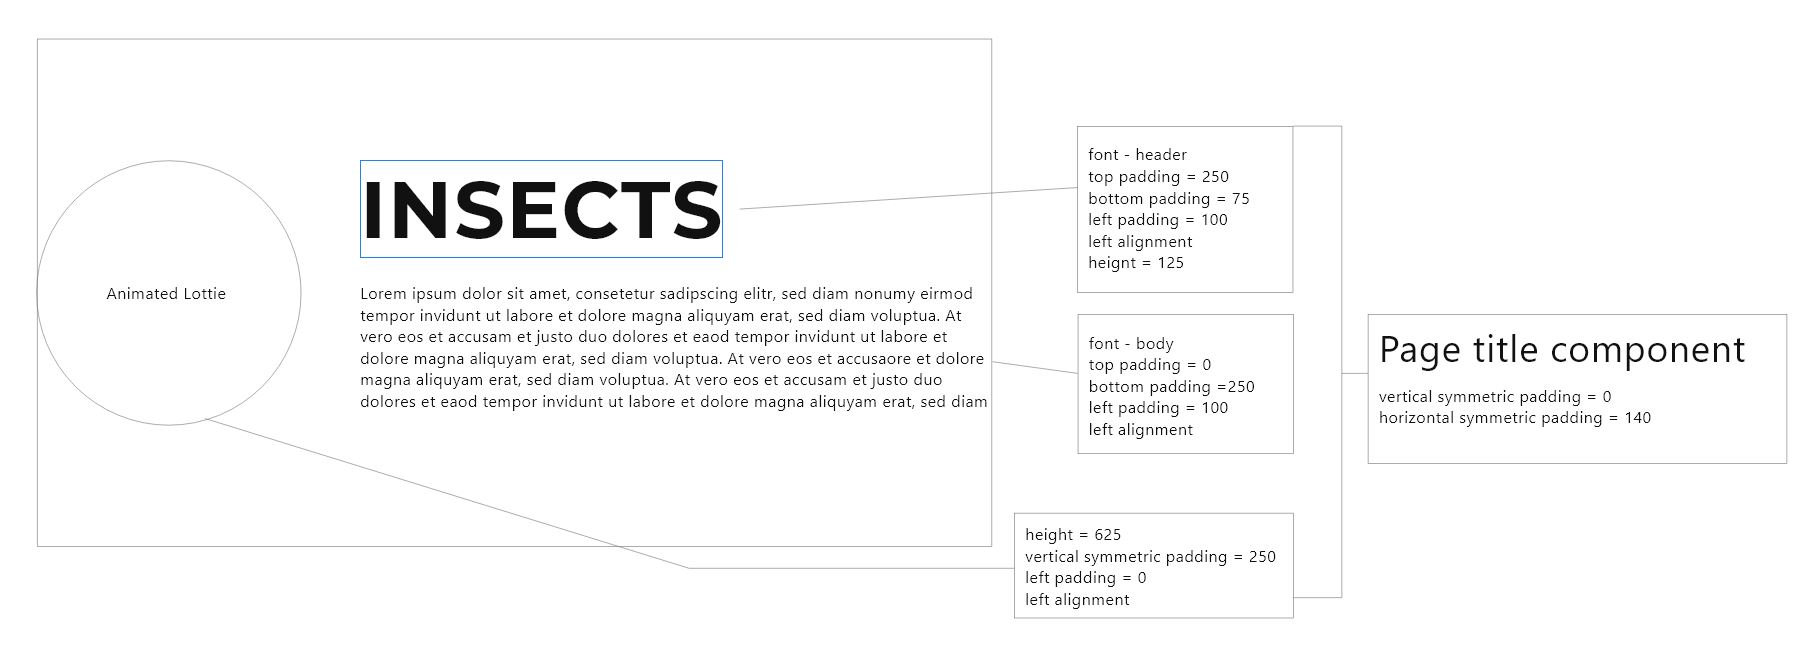
\includegraphics[scale=0.3]{Figures/wireframe-1.JPG}
		\caption{Wireframe a single title component}
		\label{fig:rb}
	\end{center}
\end{figure}

This wireframe design is then used as a point of reference to develop the website using web-technologies like React, TailwindCSS..etc and the below figure is a result of that.

% \paragraph*{Figure} Wireframe of insects page [Figure \ref{fig:rb}]
\begin{figure}[h]
	\begin{center}
		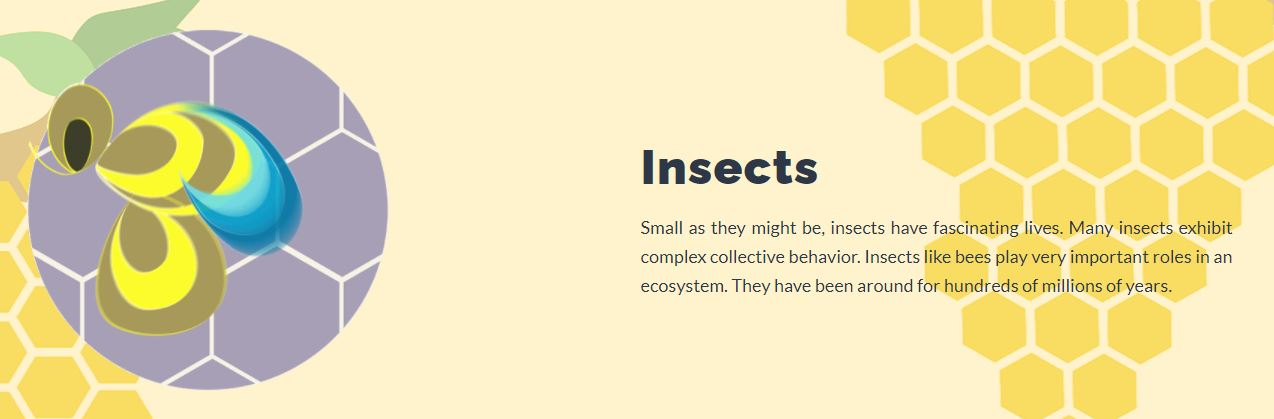
\includegraphics[scale=0.3]{Figures/insects-title.JPG}
		\caption{Wireframe a single title component}
		\label{fig:rb}
	\end{center}
\end{figure}


\section{Prototype \& testing}





